 \documentclass[11pt, twocolumn]{article}
%\documentclass[11pt,journal, compsoc]{IEEEtran}
\usepackage[utf8]{inputenc}
\usepackage{caption}
\usepackage{graphicx}
\usepackage{lipsum}
\usepackage{amssymb}
\usepackage{amsmath}
\usepackage{mathtools}
\usepackage{amsfonts}
\usepackage{bbold}
\usepackage{array}
\usepackage{xcolor}
\usepackage{cite}
\usepackage{float}
\usepackage{titling}
\usepackage{abstract}

\usepackage[top=2cm, bottom=2cm, left=1.5cm, right=1.5cm]{geometry} %choix de la taille des marges
\setlength{\droptitle}{-5em}
\usepackage{enumitem} % Pour réduire le spacing des itemize

%\textheight 22.0 cm
%\textwidth 17.0 cm
%\setlength{\oddsidemargin}{0.0cm}
%\setlength{\evensidemargin}{0.0cm}  
%\setlength{\voffset}{0.0cm}
%\setlength{\parindent}{0.5cm}
%\headheight = 20pt
%\headsep = 10pt
%\marginparsep 0pt
%\topmargin 0.0pt
%\baselineskip 14pt
%\parskip 6pt
%\footskip = 27pt
\usepackage{tikz}
\usetikzlibrary{decorations.pathreplacing}
\usetikzlibrary{patterns}
\usetikzlibrary{shapes,arrows,positioning,calc}
\tikzset{
block/.style = {draw, fill=white, rectangle, minimum height=3em, minimum width=3em},
tmp/.style  = {coordinate}, 
sum/.style= {draw, fill=white, circle, node distance=1cm},
input/.style = {coordinate},
output/.style= {coordinate},
pinstyle/.style = {pin edge={to-,thin,black},},
rectangle connector/.style={
        connector,
        to path={(\tikztostart) -- ++(#1,0pt) \tikztonodes |- (\tikztotarget) },
        pos=0.5
    },
    rectangle connector/.default=-2cm,
    straight connector/.style={
        connector,
        to path=--(\tikztotarget) \tikztonodes
    }
}

\title{\textbf{Augmented instruments : active control of a Tom Drum}}
\author{A. Caillon, J.-B. Dakeyo, M. Fouilleul, V. Fraisse, Th. Geoffroy}


\begin{document}
%\tableofcontents % A virer plus tard
\maketitle

%\IEEEtitleabstractindextext{%
%\begin{abstract}
 
%\end{abstract}}
%\maketitle
%\IEEEpeerreviewmaketitle
%\IEEEdisplaynontitleabstractindextext

%\onecolumn
\begin{abstract}

 Active control of a musical instrument consists of adding a control-loop to an existing instrument, in order to modify its behaviour in real-time. In this project, we will focus on a percussion instrument: a tom-tom drum, consisting of a wooden shell, a batter head and a resonant head. The objective is to perform active control of the drum head by integrating the instrument in a real-time feedback system, based upon a loudspeaker that replaces the resonant head, and a microphone inserted into the drum vessel.

\end{abstract}

\section*{Introduction}

The aim of this project is to design and test a control-system, based on the replacement of the resonant head of a tom drum by a loudspeaker, driven by a computer which transforms the pressure signal measured by a microphone placed inside the cavity of the instrument.
The control algorithm embedded in the computer could allow to modify the sonic properties of the instrument.

Several aspects need to be considered for this project, with regard to both the vibration of the model of the coupled shell and membrane, and the design of the control system which allows to change certain parameters of the sound, e.g. the first resonance frequency of the system. Aspects regarding the programming of the micro-computer with real-time constraints will need to be considered, as well as the characteristics of the electroacoustic transducers involved, i.e. the loudspeaker and the microphone. Before implementing this control over a real instrument, a simulation could allow for the testing of the established control law.

This paper is organized as follows : a \textbf{state of the art} will briefly resume the usual acoustic model of a membrane coupled with a cavity, and the main principles of active control of vibration and noise. Then, the \textbf{identification of the parameters} of the loudspeaker and the membrane, and the experiments made to do so, will be summarized. These measures will be useful to characterize constants in the \textbf{model} of the total coupled system, that will be used for the %\textbf{simulation} and the 
\textbf{control} equations and algorithms. The work leading up to the \textbf{experiment} and its conditions will also be presented, including the system design and its construction. The results will be presented in a final \textbf{discussion \& conclusion}.

\section{State of the art}
\subsection{Acoustic model}
\label{AcouModel}

\paragraph{Circular Membrane}
\label{circucu}
For a circular membrane with a fixed rim at radius $r=a$, with a homogeneous tension and following the hypothesis of linear displacements, the Helmholtz equation in cylindrical coordinates is:
\begin{align}
\frac{\partial^2\eta}{\partial r^2}+\frac{1}{r}\frac{\partial\eta}{\partial r}+\frac{1}{r^2}\frac{\partial^2\eta}{\partial \theta^2}+k^2\eta = 0,
\label{eq_circular_membrane}
\end{align}

where $\eta$ is the displacement of the membrane, $k$ the wave number and $r$ the celerity of transversal waves in the membrane. We are looking for solutions of the following form:
$$
\eta = R(r)\Theta(\theta) \quad\quad \text{with }R(a)=0
$$

The solutions, detailed in \cite{fundacou} are of the following form:
$$
\begin{cases}
\Theta(\theta) = \cos(m\theta + \gamma_m)\\
R(r) = A J_m(kr)
\end{cases}
$$
with $m$ a constant, $J_m$ the \textit{Bessel functions of order m} of the first kind, and $\gamma_m$, $A$, and $B$ parameters determined by the initial conditions.

Given $j_{mn}$, the nth zero of the mth Bessel function $J_m$, we can define the wave number $k_{mn} = j_{mn}/a$, and we can write the solutions:
\begin{align}
\eta_{mn}(r, \theta, t) = A_{mn}J_m(k_{mn}r)\cos(m\theta + \gamma_{mn})e^{-j\omega_{mn} t}.
\label{displacement_memb_vide}
\end{align}

The frequencies of these modes are given by:

\begin{align}
f_{mn} = j_{mn}\frac{c}{2\pi a}.
\label{freq_propre_memb_vide}
\end{align}

\paragraph{Coupling between a membrane and a cavity}
\label{acoucoupling}

The model for a circular rim alone is not enough to properly model a drum. The coupling with the air, and most importantly the cavity plays a big part in the behaviour of the drum head. 

As presented in \cite{morse1995vibration}, when the membrane is displaced from equilibrium to the shape expressed by the function $\eta(r, \theta ,t)$, the volume of the cavity is diminished by an amount ~~$\int^{a}_{0}\int^{2\pi}_{0} \eta \: r drd\theta$.~~ Let's assume that the equilibrium volume inside the cavity is $V_0$ and the equilibrium air density is $\rho_0$. When the alternations of pressure are rapid enough to be adiabatic changes, the excess pressure inside the cavity can be expressed as a variation of the initial volume as follows : 

\begin{equation}
    p = - \Bigg(\frac{\rho_0c_a^2}{V_0}\Bigg)\int^{a}_{0}\int^{2\pi}_{0} \eta \: rdrd\theta,
    \label{pression_supp_var_vol}
\end{equation}

where $c_a$ is the velocity of sound waves in the air at the equilibrium pressure and temperature in the cavity. The pressure is expressed with a negative sign because it is always in the opposite direction to the average displacement of the membrane. Thus, the coupled equation of motion for the membrane becomes (for harmonic vibrations):

\begin{equation}
    \nabla^2\eta +k^2\eta = \Bigg(\frac{\rho_0c_a^2}{V_0}\Bigg)\int^{a}_{0}\int^{2\pi}_{0} \eta \: rdrd\theta.
    \label{eqrefmemb}
\end{equation}

If $\eta_{mn}=A_{mn}J_m(k_{mn}r)\cos(m\theta + \gamma_{mn})e^{-j\omega_{mn} t}, m > 0$, the integral on the right-hand side of this equation will be zero, and the solution that satisfies the boundary conditions will be the characteristic equation \eqref{eq_circular_membrane}. Therefore, this model assumes that the presence of the airtight cavity has no effect on the normal modes of vibration which have one or more diametrical nodal lines. 

%Based on \cite{fundacou}, given that $\mathcal{P}V^\gamma$ is constant for adiabatic changes in volume, and given that the change of volume of the entrapped air in the drum cavity $dV = \pi a^2 \langle y\rangle_s$ \footnote{with $\langle y\rangle_s$ the average instantaneous displacement of the membrane}.

%The coupling generates a force $d\mathcal{P}drd\theta$ on each incremental area $rdrd\theta$ of the membrane, with:
%$$
%d\mathcal{P} \approx -\gamma(\mathcal{P}_0/V_0)\pi a^2 \langle y\rangle_s
%$$

%The only modes affected by this force are the symmetrical modes ($m=0$), which natural frequencies can be determined by solving (per \cite{fundacou}) for $ka$:
%$$
%J_0(ka) = - \underbrace{\left( \frac{\pi a^4 \gamma \mathcal{P}_0}{\mathcal{T}V_0} \right)}_B\cdot \frac{J_2(ka)}{(ka)^2}
%$$

%The area $\pi a^2$ and the volume at rest $V_0$ are therefore parameters that can be varied to alter the resonant frequencies of the system.




%\cite{vibandsound}

\subsection{Active Control}\label{sec:activecontrol}
\subsubsection{Active Control of Vibration}

The chapter 3 of the book \cite{fuller1996active} explains how to control simple or more complex mechanical systems,  with a guaranty of stability.  For instance, several choices like the number of sensors, the feedback control approach, and others aspects influence the possibility of a correct control of an entire physical system, or just of a selected part of it.\\

\paragraph{Laplace domain approaches}

In the case of systems in which the original excitation of the structure due to the primary source cannot be directly observed, a feed-forward method cannot be implemented, and a feed-back approach is then preferred. The Figure \ref{feedback_control_system_scheme} presents the associated feedback control system.  

\begin{figure}[H]
    \centering
    \begin{tikzpicture}[auto, node distance=2cm,>=latex']
    \node [input, name=u, label=above:$F_p(s)$] (u){};
    \node [sum, right of=u] (sum) {};
    \node [left of=sum, node distance=0cm, xshift=0.25cm, yshift=-0.25cm] (plus) {\tiny{-}};
    \node [left of=sum, node distance=0cm, xshift=0.5cm, yshift=-0.65cm] (plus) {$F_s(s)$};
    
    \node [left of=sum, node distance=0cm, xshift=0.25cm, yshift=0.15cm] (plus) {\tiny{+}};
    \node [block, right of=sum, node distance=2.5cm] (top) {$G(s)$};
    \node [output, right of=top, name=y, label=above:$W(s)$, node distance=2.5cm] (y){};
    \node [block, below of=top, node distance=1.5cm] (bottom) {$H(s)$};
    
    \draw [->] (u) -- (sum);  
    \draw [->] (sum) -- (top);  
    \draw [->] (top) -- node[name=ylabel]{} (y);  
    \draw [->] (ylabel) |- (bottom);  
    \draw [->] (bottom) -| (sum);  
    \end{tikzpicture}
    \caption{Classical feedback loop method}
    \label{classical_feedback_control_system_scheme}
\end{figure}


The stability for a linear single-channel feedback system can be most readily determined
by an inspection of the position of its closed loop poles. They are determined by the roots of the characteristic equation in the Laplace domain given by : $1 + G(s)H(s) = 0$ which is obtained from the closed loop transfer function equation. 
If we denote these poles and zeros respectively by the complex numbers $p_1$, $p_2 . . . $, and $z_1$, $z_2 . . .$ (i.e. the roots of $G(s)= 0$) the closed loop transfer function equation can be written as : 

\begin{equation}
\frac{W(s)}{F(s)} =  \frac{ K(s- z_1)(s- z_2)...}{(s -p_1)(s - p_2)...},
\label{transfer_function}
\end{equation}


where K is a constant gain factor. The poles and zeros in \eqref{transfer_function} are either real numbers or
conjugate pairs of complex numbers.
The impulse response can be derived by inverse Laplace transformation  to give : 

\begin{equation}
  f(t) = a_1 e^{p_1 t}  + a_2 e^{p_2 t} + ...,  
  \label{trasient_respone}
\end{equation}


where $a_1$, $a_2$, etc., are constants. The important thing to retain with the equation \eqref{trasient_respone} is that if we want f(t) to decay to zero with increasing time, the real part of each pole $p_i$ must be negative. It is a stability condition for a single-channel feedback. 
To determine these parameters, two approaches can be used: firstly a \textbf{pole-zero} representation of the individual transfer functions\footnote{e.g. the root locus method}, or a frequency response representation \footnote{e.g. the Nyquist method}.\\

However, it is also necessary to be careful about the stability of these methods, which depends on the delay and phase shifting. These phenomena may arise because of the dynamic response of the sensors or actuators used, or
may be due to time delays in the controller (if anti-aliasing and
reconstruction filters are used.).
One of the solutions is to carefully choose the feedback parameters you wish to control. For example displacement and acceleration feedback can make the system unstable by decreasing the effective damping, but it is not the case for velocity feedback.\\

\paragraph{Time domain approach}

Another method named \textbf{“State variable approach”} keeps the equations in the time domain but rewritten in terms of internal state variables of the system. The transient response of the system is now dependent on the eigenvalues of a system matrix, which must of all have a negative real part. By introducing the state variables which act as intermediate between the input signals and output signals, a broader class of behavior can be described by the simple input-output transfer function used above.  A subsystem could for instance become very large for certain excitation frequencies without significantly affecting the output of the system. The expected states control and the control stability are ensured respectively by the value and the sign of the eigenvalues of the closed loop system matrix. This approach allows to control in a different way than with the two Laplace domain approaches. \\

Moreover, with a multiple feedback channel, it is possible to control independently the different states of the system, which allow us to synthesize a mechanical system with dynamic properties that could not have been obtained by the adjustment of the system mechanical parameters.\\

%The book also talk about a special observation case, when all the state variables could not be calculated directly by operations on the outputs, a strategy which has been developed is to estimate the state variables from a limited number of observations is the state estimator or observer.
%The objective is to ensure that the internal states of the electronic state estimator, which can of course be directly measured, will track the internal states of the mechanical system, which cannot be directly measured. However it is necessary to know some more properties on the noise that could comes from the system. But if it is known, optimal estimator exists, like Kalman filter.\\
\vspace{-10 pt}
\paragraph{Modal approach}
Finally, a last approach performs feedback in the space of modal amplitudes. This strategy is called \textbf{Independent Modal-Space Control} (IMSC). This method is useful to control the system mode by mode, however it is necessary to be careful about the unmodelled modes, which might have unintended effects on the system, that could lead to instability. 

\subsubsection{Active Noise Control}

 The 1993's S.J. Elliott an P.A. Nelson article \cite{248551} provides a good overview of active noise control. Despite the fact that it mostly concerns noise cancellation, the systems that are presented in it can substantially help the understanding of active noise control. 
 
 \paragraph{Sound in enclosures}
 
 All of the strategies for active control listed in \cite{248551} rely on the principle of superposition of two sound fields that ideally result in destructive interference. For a free field situation, that goal is equivalent to a minimization of the total power output of both sources. But for a small enclosure such as the interior of a tom-tom drum, the sound field is reflected off the enclosure boundaries, causing numerous acoustical resonances (see part. \ref{AcouModel}). Nevertheless, the global effect of an active noise control system can be assessed using the total acoustic potential, that is proportional to the sum of the mean square amplitudes of each of the acoustic modes. Since this quantity turns out to be nearly proportional to the net acoustic power output of the two sources inside the enclosure \cite{elliototo}, an optimization of the noise control system is still possible by minimizing the total power output. It is not possible, in practice, to measure the total acoustic potential energy in an enclosure, but the RMS energy value of a finite number of microphone can be used as the criterion which the active control system minimizes. To do such a thing, the microphones need to be positioned in the enclosure in a way that they can be affected by all the dominant acoustic modes. 
 
 \paragraph{Feedback control}
 
 Feedback methods of active noise control are a simple way to perform active noise control. Its idealized principle is schematized in figure \ref{feedforward}, where \textit{e} represents the signal derived from the microphone, due to the combined effects of the primary disturbance that needs to be controlled, \textit{d}, and the feedback loop, which have an electrical transfer function $H$. The electrical transfer function from the corrective loud speaker input to the microphone output, that includes digital converters and anti-aliasing filters, $C$, is called the secondary path. From this conventional feedback scheme, the transfer function between disturbance and measured error is thus : 
 
 \begin{align}
     \frac{E(s)}{D(s)} = \frac{1}{1 - C(s)H(s)}.
 \end{align}
 
 \noindent
 Since the frequency response of the secondary path, $C(j\omega)$, is not perfectly flat, and furthermore contains phase shifts due, for example, to the electroacoustic response of the moving coil of the loudspeaker, or to the acoustical path between the loudspeaker and the microphone, it is not viable to introduce a negative feedback with a given gain, $H(j\omega) = -A$, in order to cancel the acoustic pressure at the monitor microphone. Indeed, as the phase shift approaches $180^\circ$, the negative feedback becomes positive, and so on, unstable. It is obvious then that a negative model could not work in high frequencies, since the acoustical path between the speaker and the microphone would introduce substantial phase shifting. 
 
 \begin{figure}[h]
     \centering
     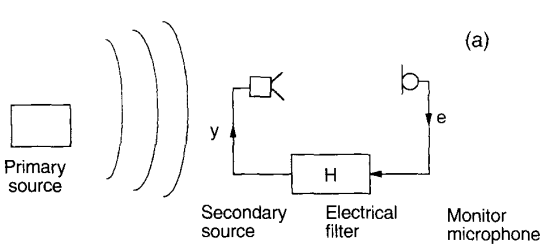
\includegraphics[width = 7 cm]{feedback_scheme.PNG}
     \caption{Active noise system using feedback control \cite{248551}}
     \label{feedforward}
 \end{figure}
\vspace{10 pt}

Nevertheless, it is possible to introduce compensating filters to correct for the phase shift in the secondary path to some extent, and increase the bandwidth over which active control is possible. If we assume that the controller is implemented as the parallel combination of a feedback path, $W$, and a feed-forward path, $\hat{C}$, the complete feedback control system becomes :

\begin{equation*}
    \frac{E(z)}{D(z)} = \frac{1 + W(z)C(z)}{1 + W(z)(\hat{C}(z) - C(z))}.
\end{equation*}

If the feed-forward part of the controller is adapted to have the same transfer function as the system under control, then the system becomes: $\frac{E(z)}{D(z)} = 1 + C(z)W(z)$. The feedback problem has thus been entirely transformed into a feed-forward problem. To minimize the error, $W(z)$ must act as an optimal predictor for the disturbance signal. For example, before control, $\hat{C}(z)$ could be adapted to model $C(z)$ and $W(z)$ could then be adapted with a copy of $\hat{C}(z)$ using the \textit{Multiple Error LMS Algorithm} described in \cite{248551} to generate the desired filtered reference signal.

\section{Identification experiments}

To control the system, we must at first identify its dynamic behaviour according to its different parts: speaker membrane, tom membrane and the inherent coupling between them. Here, we will start by analyzing the modal components of the tom membrane, to then study the physical parameters of the loudspeaker.

\subsection{Drum head parameters}

\paragraph{Conditions of the experiment}
The resonance drum head is removed, and is replaced by the rigid surface of the table the drum is clamped to\footnote{~It is noted that the presence of this rigid reflective surface almost entirely cancels the first mode of the membrane.}, in order to evaluate the response of the drum without the resonant drum head. The remaining batter drum head is uniformly tuned at each tension rod, to allow the approximation of uniform tension across the membrane, and finally a DPA-4099 microphone is inserted inside the drum, in order to measure acoustic response inside the cavity.

Then, the drum head is hit with two kinds of sticks; a standard drum stick and a kettledrum's mallet, in two positions~: once near the border of the membrane, in order to excite all resonance modes, and once in the center of it, in order to excite the axi-symmetrical modes only ($m = 0$).

A first round of measures is conducted, then a mass of 10.4g of Blu-Tack is added to the membrane, and a second round of measures is conducted. Finally, a third round of measures is conducted, with a mass of 2.1g of Blu-Tack only. 

\paragraph{Measurements analysis}
In order to accurately identify the modal parameters of the drum head coupled with its cavity, the recorded measures are analyzed with the high-resolution modal identification method \textsc{esprit} \cite{ESPRIT} yielding several resonances of the system. An example of an \textsc{esprit} identification of the resonances is showed on figure \ref{fig:ident_esprit_tom}.

\begin{figure}[!h]
    \centering
    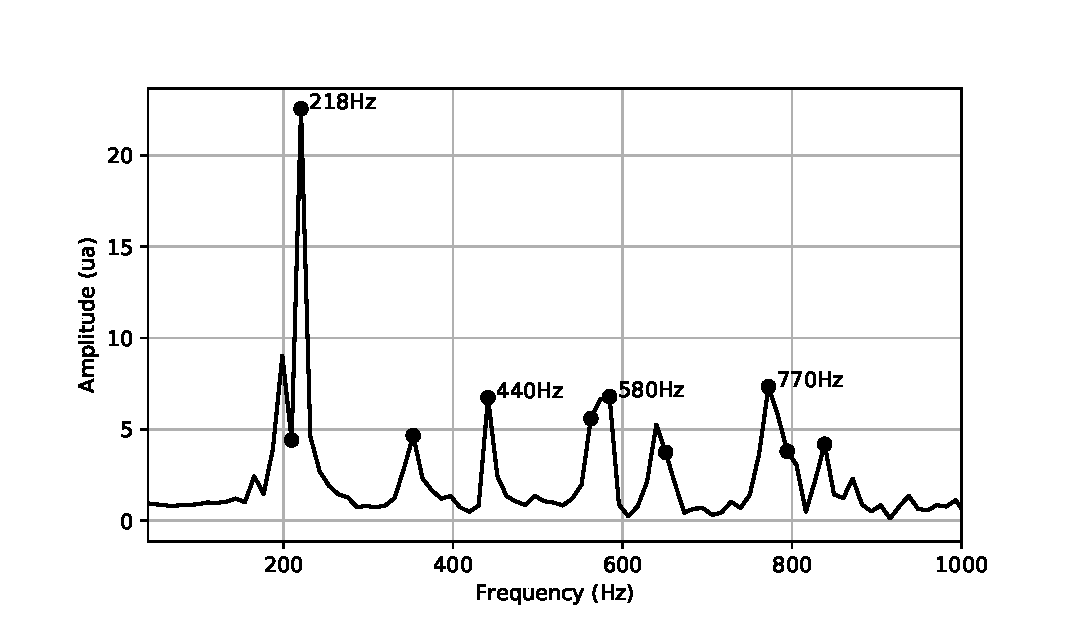
\includegraphics[width=\linewidth]{identification_esprit_tom.eps}
    \caption{Tom spectrum when softly hit, alongside poles identified by \textsc{esprit}.}
    \label{fig:ident_esprit_tom}
\end{figure}

\vspace{5pt}

The two last rounds of measures are useful to estimate parameters of the membrane such as its equivalent mass and compliance. Indeed, considering at a first order approximation the membrane as a one degree of freedom system, its resonance frequency $f_{res}$ can be seen as a variable relative to the mass $M_d$ and the compliance $C_d$ of the equivalent system :

\begin{equation}
    f_{res} = \frac{1}{2\pi \sqrt{C_d M_d}}.
\end{equation}

Adding an additional mass $m$ into such a system shifts its resonance frequency, let's call it $f'_{res}$. By comparing both resonance frequencies, it is possible to estimate the mass of the membrane:

\begin{equation}
    M_d = \frac{m}{\frac{f_{res}^2}{f'^2_{res}} - 1}.
\end{equation}

This is a first order estimation, but this will give an approximation of the surface mass of the membrane.

\paragraph{Results}

We found a mass of $10.2 \pm 0.2 g$ for $M_d$, using the third round of measures, with low resonance frequencies detected with \textsc{esprit}'s analysis.  



\subsection{Loudspeaker modeling}
\label{loudpart}

This experiment aims to identify the voltage-position transfer function of the loudspeaker that will control the system.


\paragraph{Loudspeaker dynamic}
To model the loudspeaker, we start by applying Newton's second law to the moving mass $M_m$ : 
\vspace{-.1cm}
\begin{align}
    \hspace{-20pt}M_m \Ddot{x}_{sp}(t) + R_m \Dot{x}_{sp}(t) + K_m x(t) = BLi(t) + P_{sp} S_{sp},
    \label{eq_mvt_HP_non_simplifcation}
\end{align}

 \noindent
 $B$, $L$ and $I$ are respectively the magnetic field in the loudspeaker's air gap, the length of the coil, and the current intensity inside the coil.
 Considering that the dynamic is studied on a frequency range where the sound speaker impedance $Z_{sp}$ is considered constant, the electrical current $i$ can be expressed in function of the associated tension $u$ as $i =  1/R_e *(u - Bl \Dot{x}_{sp})$, where $Bl \Dot{x}_{sp}$ is an electromotive force.
 
 
 The pressure term $P_{sp}S_{sp}$, resulting from the coupling with the cavity, can be considered an additional damping $\Delta K$ on the loudspeaker membrane. The equation becomes:
 \vspace{-0.2cm}
 \begin{align}
    \hspace{-25pt} M_m \Ddot{x}_{sp}(t) + \underbrace{R_m \Dot{x}_{sp}(t) + \mathbf{K'} x(t)}_{\text{Negligible}} = \frac{BL}{R_e} *(u - Bl \Dot{x}_{sp}).
\end{align}
 
 In the case of our loudspeaker, with regard to its frequency resonance and the frequency range which will be used, the mechanical resistance and damping term are negligible. \\

 Considering the harmonic case such that for any parameter $\alpha$, $\alpha = \Tilde{\alpha} e^{j \omega t } e^{j \phi}$, it leads to the following expression of the transfer function $H(s)$ in the Laplace domain :
 \vspace{-0.2cm}
\begin{align}
     H(s) = \frac{\tilde{X} }{\tilde{U} } (s) = 
     \frac{  e^{j \phi } }
     { ( s^2  M_m + s  (Bl)^2/R_e)}
     \label{FRF_HP_expression_nosimplification}
\end{align}
 
 
\paragraph{Conditions of the experiment}

The loudspeaker is connected to a \textit{dSPACE microlab box} codec, which is itself wired to a laser vibrometer, pointing into the loudspeaker's membrane, as schematized in figure \ref{laserexp}.

\begin{figure}[h!]
    \centering
    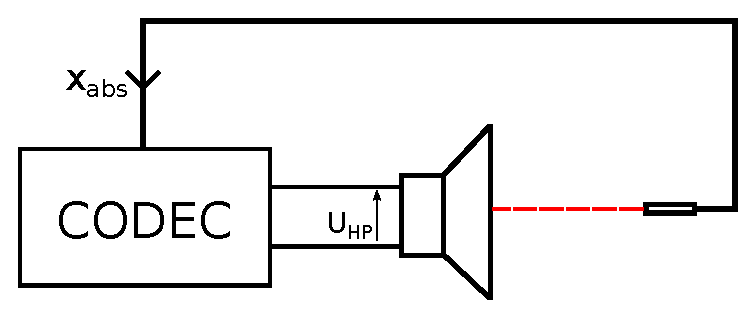
\includegraphics[width = 6cm]{lazer.eps}
    \caption{\scriptsize{Identification of the loudspeaker's transfer function}}
    \label{laserexp}
\end{figure}

Using \textit{Simulink}, a chirp signal is sent into the loudspeaker from the codec, that receives the absolute position $x_{abs}$ of the loudspeaker's membrane from the vibrometer.
The input tension $u$ at loudspeaker terminals characterized by the chirp, and the real output displacement given by $x_{sp} = x_{abs} - x_{mean}$, are related by $h(t)$ as expressed in equation \eqref{displacment_hp_expression} : 
\begin{align}
    x_{sp}(t) = h(t) * u(t),
    \label{displacment_hp_expression}
\end{align}

\paragraph{Response identification} The equation \eqref{FRF_HP_expression_nosimplification} shows that the frequency response of the sound speaker is a two-pole filter, which can be approximated by an second order auto-regressive filter (AR2).
Considering this identified filter, we can construct the inverse filter $h^{-1}$ as a second order Moving Average (MA2) filter, to whiten the frequency response of our loudspeaker, governed by the following recurrence equation : 
\begin{align}
    x[n] = a_0 \: u[n] + a_1 \: u[n-1] + a_2 \: u[n-2],
\end{align}

with $a_0$, $a_1$ and $a_2$, the three coefficients, estimated by a method using Yule-Walker equations \cite{cours_fpa_tns}.
While the identification of the parameters $M_m$ and $(Bl)^2/R_e$ would call for setting $a_0$ to be strictly null, our use case merely requires the whitening of the voltage-position transfer function of the loudspeaker.
\noindent
Figure \ref{fig:fig_frf} shows the result of the corrective MA2 filter on the loudspeaker's response.

\begin{figure}[H]
    \centering
    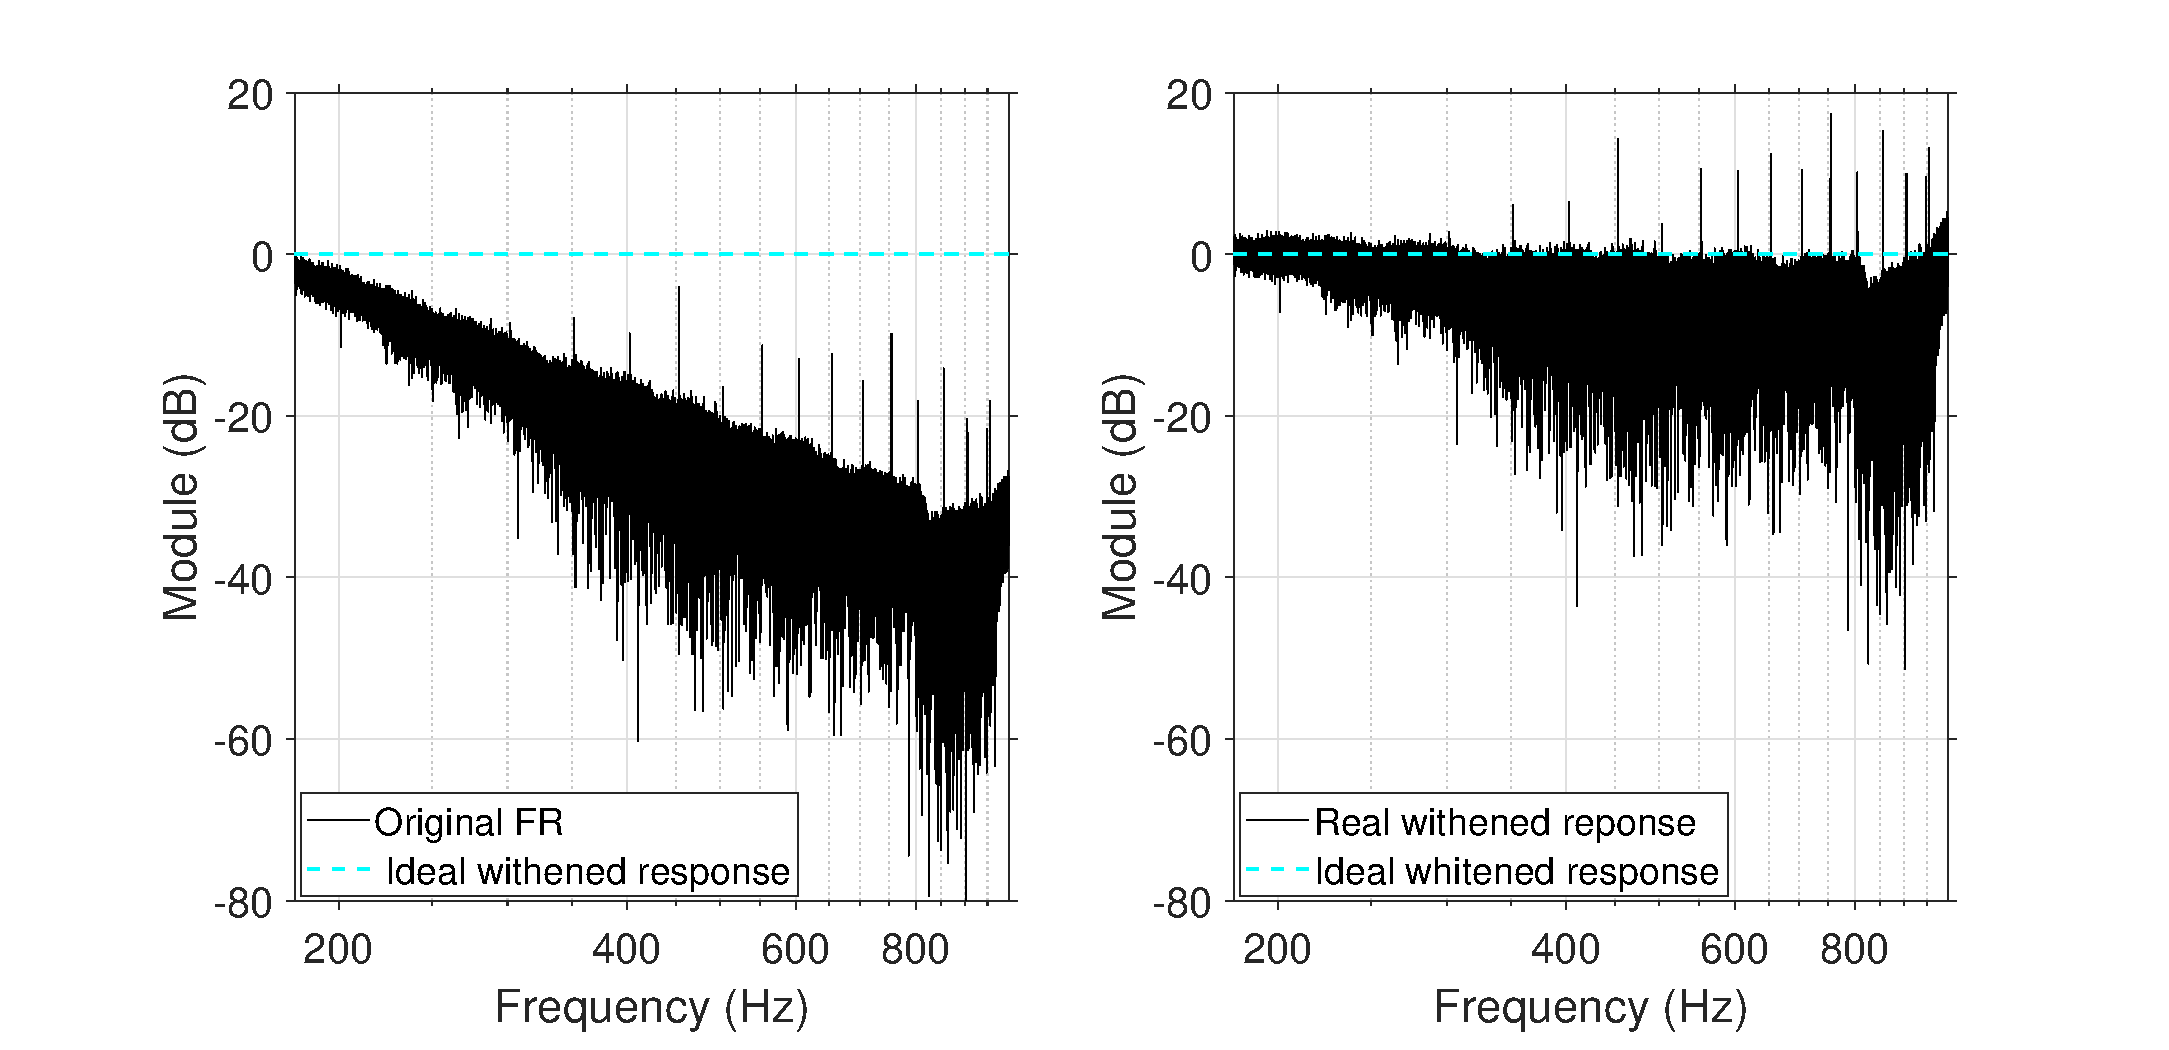
\includegraphics[scale= 0.25]{compar_FRF_avec_withened_FRF_HP.eps}
    \caption{Original and whitened frequency response of the loudspeaker voltage-position transfer function}
    \label{fig:fig_frf}
\end{figure}

\section{Physical model}\label{physical_model}

The objective now is to model the entire system, from the loudspeaker's command to the membrane, considering the microphone's observation.
\paragraph{Continuous equations}
The membrane's model is inspired by the document \cite{morse1995vibration}, considering a coupling between the movement of the loudspeaker, the drum's vessel and the membrane itself. This model takes care about few more hypotheses. First, the non axi-symmetric head drum modes ($m > 0$) are ignored, because of their total volume variation. Actually, it has been explained in \cite{morse1995vibration} that, if the total volume is always conserved, these modes are not useful in our approach to illustrate the coupling between cavity and membrane. Moreover, if only the axi-symmetric modes are modeled, the displacement $\eta$ is not function of $\theta$, because of a symmetric revolution.

Concerning the loudspeaker, its membrane displacement $x_{sp}$ is approximated by a plate piston of area $A_{sp}$ which creates, in the same way as the tom membrane, a variation of the initial volume inside the cavity.  Considering all these hypotheses, another pressure term appears in the equation \eqref{eqrefmemb} which becomes:

\begin{align}
    \nabla^2 \eta +\frac{1}{c^2}\ddot \eta = \Bigg(\frac{\rho_0c_a^2}{V_0}\Bigg)  \left[ 2 \pi \int^{a}_{0} \eta \: rdr +
    A_{sp} \: x_{sp}       \right].
\end{align}

\noindent
What we are interested in at this step is the time evolution of $\eta$. Indeed, the excess pressure in the cavity changes only the time evolution of $\eta$, that means the head drum eigen-frequencies are not the same anymore, but the modal shapes don't change. Thus it is useful to set a variable separation $\eta(r,t) = \Phi (r) \: \tilde{\eta}(t)  $. Considering a projection in the modal base of $\phi(r)$ which is deduced from \eqref{displacement_memb_vide}, the membrane's displacement $\tilde{\eta}$ is solution of:

\begin{align}
    \Ddot{\Tilde{\eta}} + \frac{C}{M} \Dot{\Tilde{\eta}} + \frac{K}{M} \Tilde{\eta} = \frac{\beta}{M} f(x_{sp})\delta(t - t_1),
    \label{equ_displa_modal}
\end{align}

\noindent
where M, C and K are respectively the modal mass, damping and stiffness of the membrane coupled with the cavity. The right-hand side of the equation models the equivalent force applied from the loudspeaker. It should be noted that $\beta$ is an arbitrary constant taking into account the acoustic impedance break between the loudspeaker membrane and the tom membrane, and that $\delta(t - t_1)$ stands for a time delay that comes from the acoustical path between both membranes. $f(x_{sp})$ models the acoustical pressure force at the speaker membrane level relative to its displacement $x_{sp}$, using the same kind of development done in \cite{morse1995vibration}: 

\begin{equation}
    f(x_{HP}) = S_{sp} P_{sp}(x_{sp}) = \Bigg(\frac{\rho_0c_a^2}{V_0}\Bigg) S_{sp}^2 x_{sp}.
\end{equation}

\vspace{5pt}
\noindent

The three modal parameters on the left-hand side of \eqref{equ_displa_modal} are relative to the eigen-frequencies of the membrane which are :

\begin{equation}
    f_n = \frac{c}{2 \pi a} \mathcal{P}_n \bigg[ \frac{\rho c^2 a^2}{(V_0 -  A_{sp} \: x_{sp}) T} \bigg],
\end{equation}

\noindent
$\rho$, $c$, $T$ are respectively the density, transverse velocity and tension of the membrane. The $\mathcal{P}_n$ function can be retrieved by tracking the following equation's n-th root according to $\omega$ with a 4-th order polynomial, in a similar analysis to \cite{morse1995vibration}: 

\begin{align}
    J_0(\omega)  +\frac{\chi}{w^2} J_2(\omega) = 0, ~&\chi=\frac{\pi \rho c^2 a^4}{VT}, ~\omega = \frac{2\pi f a}{c}
\end{align}


\noindent
Finally, considering that the principle of linear superposition is verified, the microphone in the system returns a voltage quantity that is a function $h_n$ of the acoustical pressure inside the drum's vessel, that itself is a superposition of the acoustic waves of both membranes:

\begin{align}
    y(t) &= h_n \bigg[ \frac{\rho_0 c_a^2}{V_0} A_{sp} \: x_{sp}(t) \nonumber \\
    &+ \frac{\rho_0 c_a^2}{V_0} 2 \pi \Tilde{\eta}(t) \int_0^a \Phi(r) \: r dr  \bigg],
    \label{eq_observation_y}
\end{align}

were $\tilde{\eta}(t)$ is solution of equation (\ref{equ_displa_modal}). The two elements on the right-hand side of the equation represent the acoustic contribution of the loudspeaker and that of the drum's membrane. Phase variations and time delays induced by electronic circuits and digital conversion have not been included in the model.

%\paragraph{Numerical estimation}There are no analytic solutions for the equation \eqref{equ_displa_modal}, but the membrane's movement can be emphasized with a second order finite differences approximation : 

%\begin{align}
%    \Tilde{\eta}_+ &= \frac{\Delta t^2}{M} \bigg( \beta M_m \: \ddot X * z^{-n_1} \nonumber \\
%    &- \frac{c}{\Delta t}(\Tilde{\eta} - \Tilde{\eta}_-) - K \Tilde{\eta} \bigg) + 2 \Tilde{\eta} - \Tilde{\eta}_-
%\end{align}

%\noindent
%In order to properly estimate the membrane's movement, 2 samples are, thus, required. 



\section{Control Model}

The aim of the control is to monitor the head drum displacement, using a target $\tilde{\eta}_{des}$ and a desired tension at the loudspeaker terminals $u_{des}$. In order to this, a modal approach will be used to obtain a relation between $u_{des}$, $\tilde{\eta}_{des}$, $\tilde{\eta}_{mes}$, the desired frequency and damping. We will consider only the truncation of $\eta$ to the first mode, it implies $\eta = \eta_1$ and $y = y_1$, thus only one mode will observed and controlled .

\subsection{Design of the monitoring model}
\paragraph{Measured displacement}

To control the coupled system, a measure of the head drum displacement is needed. This is computed from the pressure measured with the microphone, according equation \eqref{eq_observation_y}, with the approximation $\tilde\eta(t) \approx \tilde\eta_{0,1}(t)$.

To express $\tilde{\eta}(t)$ we must estimate the integral along the modal shape $\phi_1(r)$, which is a first order Bessel function. According to \cite{morse1995vibration}, and from an expression of $J_m(\frac{2 \pi \nu r}{c})$, 
it leads to :

\begin{align}
        &\tilde{\eta}(t) =  \frac{1}{ 2 \pi \mathcal{B}} \Bigg[ \frac{V_0}{\rho_0 c_a^2 } y(t)  - S_{sp} \: x_{sp}(t)  \Bigg] \qquad \\ &\text{with}~~\mathcal{B} = \int_0^a r \: e^{\alpha r} \: r dr = \frac{a}{\alpha} e^{\alpha a} - \frac{1}{\alpha^2} (e^{\alpha a} - 1 ).
\end{align}

\paragraph{Continuous equations} Following the hypothesis mentioned above, the aim of the monitoring model is to establish a relation between the input voltage $u$ and the membrane temporal displacement. The latter can be find using the equation (\ref{equ_displa_modal}) and the loudspeaker modeling : 

\begin{equation}
    \Ddot{\Tilde{\eta}} + \frac{C}{M} \Dot{\Tilde{\eta}} + \frac{K}{M} \Tilde{\eta} = \frac{\beta}{M} \Bigg(\frac{\rho_0c_a^2}{V_0} S_{sp}^2 \cdot h * u \Bigg),
    \label{cacapipi}
\end{equation}

were the time delay is neglected. Using the principle of PID control \cite{PID}, it is possible to model an error dynamic $\varepsilon = \tilde{\eta} - \tilde{\eta}_{des}$ so as: 

\begin{align}
    &\Ddot{\varepsilon} + \lambda_1 \Dot{\varepsilon} + \lambda_2 \varepsilon = 0 \nonumber\\
    \iff &\Ddot{\tilde{\eta}} = \Ddot{\tilde{\eta}}_{des} - \lambda_1 (\dot{\tilde{\eta}} - \dot{\tilde{\eta}}_{des}) - \lambda_2 (\tilde{\eta} - \tilde{\eta}_{des}).
\end{align}

From this equation, and by injecting $\Ddot{\tilde{\eta}}$ in the equation (\ref{cacapipi}), we have :

\begin{align}
    &\Ddot{\tilde{\eta}}_{des} + \lambda_1 \dot{\tilde{\eta}}_{des} - \lambda_1 \dot{\tilde{\eta}} + \lambda_2 \tilde{\eta}_{des} - \lambda_2 \tilde{\eta} + \frac{C}{M} \dot{\tilde{\eta}} + \frac{K}{M} \tilde{\eta} \nonumber \\
    &= \frac{\beta}{M} \Bigg(\frac{\rho_0c_a^2}{V_0} S_{sp}^2 . h * u \Bigg).
\end{align}

Knowing that the tom membrane is modelled by a system with one degree of freedom, we have:

\[
\left\{
\begin{array}{r c l}
\frac{C}{M} &=& 2 \xi \omega\\
\\
\frac{K}{M} &=& \omega^2
\\
\text{And we set }\gamma &=& \Big(\frac{\rho_0c_a^2}{V_0} S_{sp}^2 \Big)
\end{array}
\right.
\]

 Finally, we get an equation linking the input tension and the desired membrane displacement : 

\begin{align}
    u &= h^{-1} * \Bigg( \frac{1}{\gamma} \Big[ \Ddot{\tilde{\eta}}_{des} + \dot{\tilde{\eta}} (2 \xi\omega - \lambda_1) \nonumber \\
    & + \tilde{\eta} (\omega^2 - \lambda_2) + \lambda_1 \dot{\tilde{\eta}}_{des} + \lambda_2 \tilde{\eta}_{des} \Big] \Bigg),
    \label{continuous_control}
\end{align}


with $h^{-1}$ the inverse impulse response of the loudspeaker, as described in part \ref{loudpart}.

\paragraph{Numerical implementation} 

In order to implement a monitoring algorithm based on the equation (\ref{continuous_control}), a computation of the desired displacement of the tom's membrane $\tilde{\eta}_{des}$ is needed. Thus, during an observation of the actual membrane displacement $\tilde{\eta}$ at a given discretized time $n$, two samples of $\tilde{\eta}_{des}$ are computed, one for the actual observation time $\tilde{\eta}_{des}^n$, and one for the next time sample $\tilde{\eta}_{des}^{n+1}$. The first is calculated from two previous observations $\tilde{\eta}^{n-1}$ and $\tilde{\eta}^{n-2}$ while the second is calculated from $\tilde{\eta}_{des}^n$ and the previous observation $\tilde{\eta}^{n-1}$. The desired displacement is supposed to be a damped harmonic oscillator :

\begin{equation}
    \Ddot{\tilde{\eta}}_{des} + 2 \xi \omega \dot{\tilde{\eta}}_{des} + \omega^2 \tilde{\eta}_{des} = 0,
\end{equation}

and is estimated with a second order finite difference approximation :

\[
\left\{
\begin{array}{r c l}
\Ddot{\tilde{\eta}}_{des}^n &=& \frac{1}{\Delta t^2} [\tilde{\eta}_{des}^{n+1} + \tilde{\eta}^{n-1} - 2 \tilde{\eta}_{des}^n ]\\
\\
\dot{\tilde{\eta}}_{des}^n &=& \frac{1}{\Delta t} [\tilde{\eta}_{des}^n - \tilde{\eta}^{n-1}]\\
\end{array}
\right.
\]

where $\Delta t$ is a sample period. We have :
{\small
\begin{align}
    \hspace{-20pt}\tilde{\eta}_{des}^n &= \Delta t^2 \bigg(- \frac{2\xi\omega}{\Delta t} (\tilde{\eta}^{n-1} - \tilde{\eta}^{n-2}) - \omega^2 \tilde{\eta}^{n-1} \bigg) - \tilde{\eta}^{n-2} + 2\tilde{\eta}^{n-1} \nonumber\\
    \hspace{-20pt}\tilde{\eta}_{des}^{n+1} &= \Delta t^2 \bigg(- \frac{2\xi\omega}{\Delta t} (\tilde{\eta}_{des}^{n} - \tilde{\eta}^{n-1}) - \omega^2 \tilde{\eta}_{des}^{n} \bigg) - \tilde{\eta}^{n-1} + 2\tilde{\eta}_{des}^{n}. 
\end{align}
}

Finally, the monitoring algorithm can be computed from the observed and the computed displacements and their derivatives: 

\begin{align}
    u &= h^{-1} * \Bigg[\frac{1}{\gamma} \bigg( \frac{1}{\Delta t^2}(\tilde{\eta}_{des}^{n+1} + \tilde{\eta}^{n-1} - 2 \tilde{\eta}_{des}^n) \nonumber \\
    &+  \frac{1}{\Delta t} (\tilde{\eta}^n - \tilde{\eta}^{n-1})[2\xi\omega - \lambda_1] + \tilde{\eta}^n(\omega^2 - \lambda_2) \nonumber \\
    &+ \lambda_1 (\frac{1}{\Delta t} (\tilde{\eta}_{des}^n - \tilde{\eta}^{n-1})) + \lambda_2 \tilde{\eta}_{des}^n \bigg)\Bigg]
\end{align}

\section{Experiment}
\subsection{Construction of the system enclosure}
In order to fasten the tom to the loudspeaker and also to alleviate the radiation from the back of the speaker, we embedded the speaker in a box, made with melamine boards, which interior was covered in absorbing foam. To get the whole system at a reasonable playing height, we built the box 70cm tall. It also features external banana connectors to connect the external amplifier to the speaker. The tom drum, once rid of its resonance head and lower rim, is screwed to the box top, on top of the speaker, with a \textsc{plastiline®} seal applied to every gap to ensure the air-tightness of the build. Figure \ref{fig:cross_sec} shows a cross-section of the system. An overview is available at the appendix.

\begin{figure}[H]
    \centering
    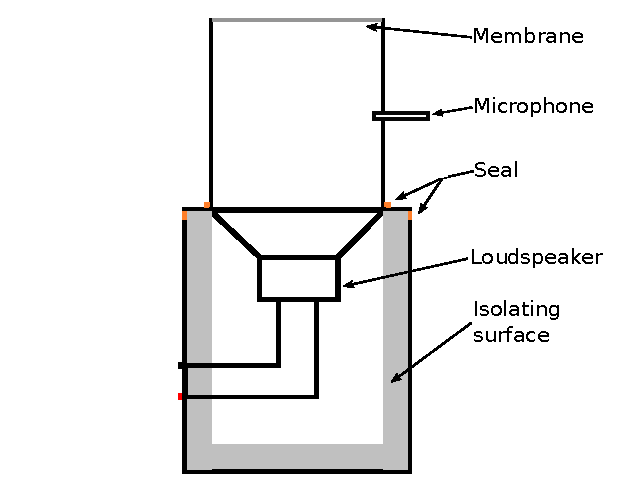
\includegraphics[width=0.7\linewidth]{sys_scheme.eps}
    \caption{Cross-section of the system}
    \label{fig:cross_sec}
\end{figure}

\subsection{Physical setup}
In order to achieve active control, we need a closed feedback loop with precise timing.

We used a \textsc{bruel \& kjaer (b\&k) 4939} microphone wired to a \textsc{b\&k 2669} pre-amp and a \textsc{b\&k nexus 2692} conditioner. The monitoring system was a \textsc{coala}\footnote{~https://forge.ircam.fr/p/real$\_$time$\_$control/}, and the loudspeaker a \textsc{Raveland axx-1212} sub-woofer wired to a \textsc{phonic max 500} power amplifier.

\begin{figure}[H]
    \centering
    \begin{tikzpicture}[auto, node distance=2cm,>=latex']
    \node [input, name=u, label=above:$p_h$] (u){};
    \node [sum, right of=u] (sum) {};
    \node [left of=sum, node distance=0cm, xshift=0.25cm, yshift=-0.25cm] (plus) {\tiny{-}};
    \node [left of=sum, node distance=0cm, xshift=0.5cm, yshift=-0.65cm] (plus) {$p_s$};
    
    \node [left of=sum, node distance=0cm, xshift=0.25cm, yshift=0.15cm] (plus) {\tiny{+}};
    \node [block, right of=sum, node distance=4cm] (top) {Mic};
    \node [output, right of=top, name=y, label=above:$y$, node distance=3.5cm] (y){};
    \node [block, below of=top, node distance=1.5cm, xshift=1cm] (coala) {\textsc{coala}};
    \node [block, left of=coala] (amp) {Amp};
    \node [block, left of=amp] (spkr) {Speaker};
    \draw [->] (u) -- (sum);  
    \draw [->] (sum) -- (top);  
    \draw [->] (top) -- node[name=ylabel]{} (y);  
    \draw [->] (ylabel) |- (coala);
    \draw [->] (coala) -- (amp);
    \draw [->] (amp) -- (spkr);
    \draw [->] (spkr) -| (sum);  
    \end{tikzpicture}
    \caption{Feedback loop}
    \label{feedback_control_system_scheme}
\end{figure}


\subsection{COALA}
\subsubsection{Reconfiguring the COALA OS}
The \textsc{coala} is an embedded linux machine, based on the Beaglebone Black and a custom cape that integrates a precision ADC and a precision DAC, in conjunction with a preamp and a power amplifier.

The unit we got\footnote{\textsc{coala} \textit{Alto}} was misconfigured, and therefore inaccessible by SSH.

By cloning the OS of a well-configured \textsc{coala} unit\footnote{\textsc{coala} \textit{Cello}}, we were able to access the unit, and change the following configuration files:
\vspace{-0.15cm}
\begin{itemize}[noitemsep]
    \item \texttt{/etc/hostapd/hostapd.conf}
    \item \texttt{/etc/dhcpd/dhcpd.conf}
    \item \texttt{/etc/network/interfaces}
\end{itemize}
%\vspace{-0.1cm}
which respectively configure the local wireless access-point the machine generates, the DHCP service necessary for the proper operation of \texttt{hostapd}, and the \textsc{coala}'s static IP adress.

\subsubsection{Rewiring the \textsc{coala} signal path}
By default, the \textsc{coala} is equipped with a DIP switch (see Figure \ref{fig:coala_switch}), accessible on the front of the enclosure. This allows for several different configurations, the most common being 2--7, which is to say:
$$
\boxed{Preamp_{out}} \longrightarrow \boxed{ADC_{in}}
\quad \& \quad
\boxed{DAC_{out}} \longrightarrow \boxed{Amp_{in}}
$$
\begin{figure}[h]
    \centering
    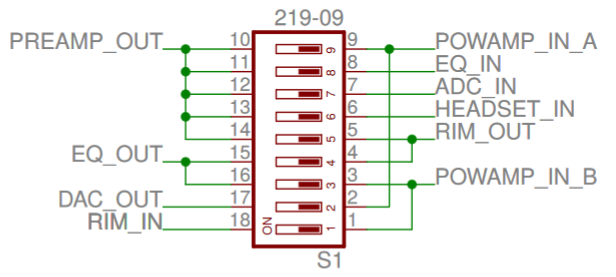
\includegraphics[width=\linewidth]{coala_switch.PNG}
    \caption{Default DIP switch wiring}
    \label{fig:coala_switch}
\end{figure}

However, none of the configurations allow for the simple configuration needed for our project, which is:

$$
\boxed{Ext_{in}} \longrightarrow \boxed{ADC_{in}}
\quad \& \quad
\boxed{DAC_{out}} \longrightarrow \boxed{Ext_{out}}
$$
In order to achieve this configuration, we need to pop the DIP switch out, and rewire manually, as shown in Figure \ref{fig:coala_rewire}.


\begin{figure}[!h]
    \centering
    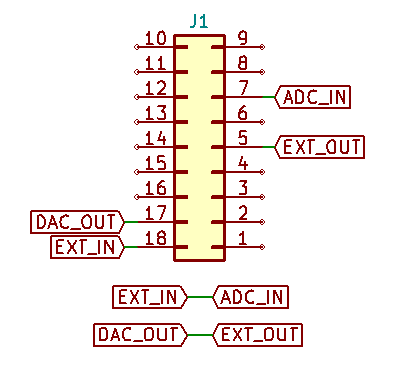
\includegraphics[height=5cm]{coala_switch_fix.PNG}
    ~
    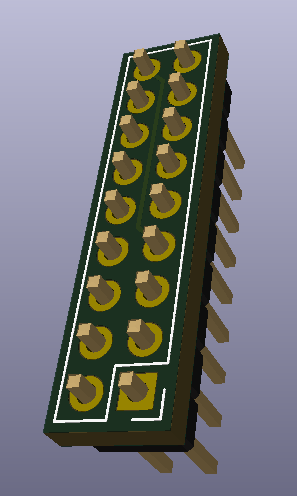
\includegraphics[height=5cm]{coala_switch_fix_render.PNG}
    \caption{Rewiring schematic and 3D rendering of the PCB}
    \label{fig:coala_rewire}
\end{figure}


\subsubsection{Programming the control law}

The \textsc{coala} codebase is mainly written in C and C++. We had the choice of using \texttt{gen\~}, a sample-accurate subsystem of Max/MSP, however coding directly in C++ seemed more flexible. 

In order to program our control law to be executed by the \textsc{coala}, we coded a class that inherits the \texttt{Filter} interface. Its \texttt{step()} method gets called each time the audio thread needs to compute a new audio sample. In this method, we first filter the input signal with a low pass biquad to keep the first mode and eliminate the higher modes of the drum head. Then we compute the control according to our control law. We finally filter it with the inverse of the speaker\'s frequency response, which we approximated by a fourth order FIR filter, before sending it to the output.

\section{Discussion}

The overall system, after the implementation of the control algorithm, doesn't work properly.
 
One culprit in the poor controllability level of the system is the overall observability, which is much restrained with merely one pressure sensor, from which is derived an estimator of the membrane displacement, which would be far better measured with a laser vibrometer, for example.

The estimator is based on several rough approximations, e.g. $\tilde\eta \approx \tilde\eta_{(0,1)}$, a model of sources superposition which is probably too simplistic to allow for a real identification of the batter head displacement, a disregard for phase shifting due to both the acoustic path and the electronic path, and a loudspeaker modeling which doesn't take in account the pressure force exerted by the cavity.

The physical model is also probably rough in terms of the precision of the measurements of the tom-tom drum's parameters, i.e. its dimensions, inner volume, batter head mass, etc.

An other potential reason for the failure of the membrane displacement control may be the lack of robustness to a variable or poorly defined loudspeaker amplifier gain. It is thus impossible for the control model to anticipate the exact sound pressure level emitted by the loudspeaker.

\section{Conclusion}

Despite the fact that an active control of the membrane displacement hasn't be achieved, several positive outcomes are to be acknowledged.

Firstly, the experiment was not strictly a failure, as an interactivity between the membrane tension evolution and the sound emitted by the loudspeaker has been observed. 

A lot of the spadework for future improvements of the systems has been done, both theoretically regarding the acoustic and control models, but most importantly \textit{technically}, thanks to the construction of the enclosure, the development of a control loop with the \textsc{coala} boards, as well as the experimental design.

Overall, the results are very encouraging, and pave the way for future developments and refinements in the models and measurements, which we are confident could be successful in achieving active control of a tom drum.

\section*{Acknowledgements}
We would like to thank Marc Wijnand, Brigitte d'Andréa-Novel and Benoit Fabre, for their supervision and support in this endeavour.

We would also like to show our gratitude to Djellal Chalabi, Camille Dianoux, Robert Piéchaud, and Tristan Lebrun, who provided insight and expertise that greatly assisted this project.

\bibliography{refs.bib}{}
\bibliographystyle{plain}
\newpage
\onecolumn
\begin{appendix}
\section*{Appendix}
\begin{figure}[H]
    \centering
    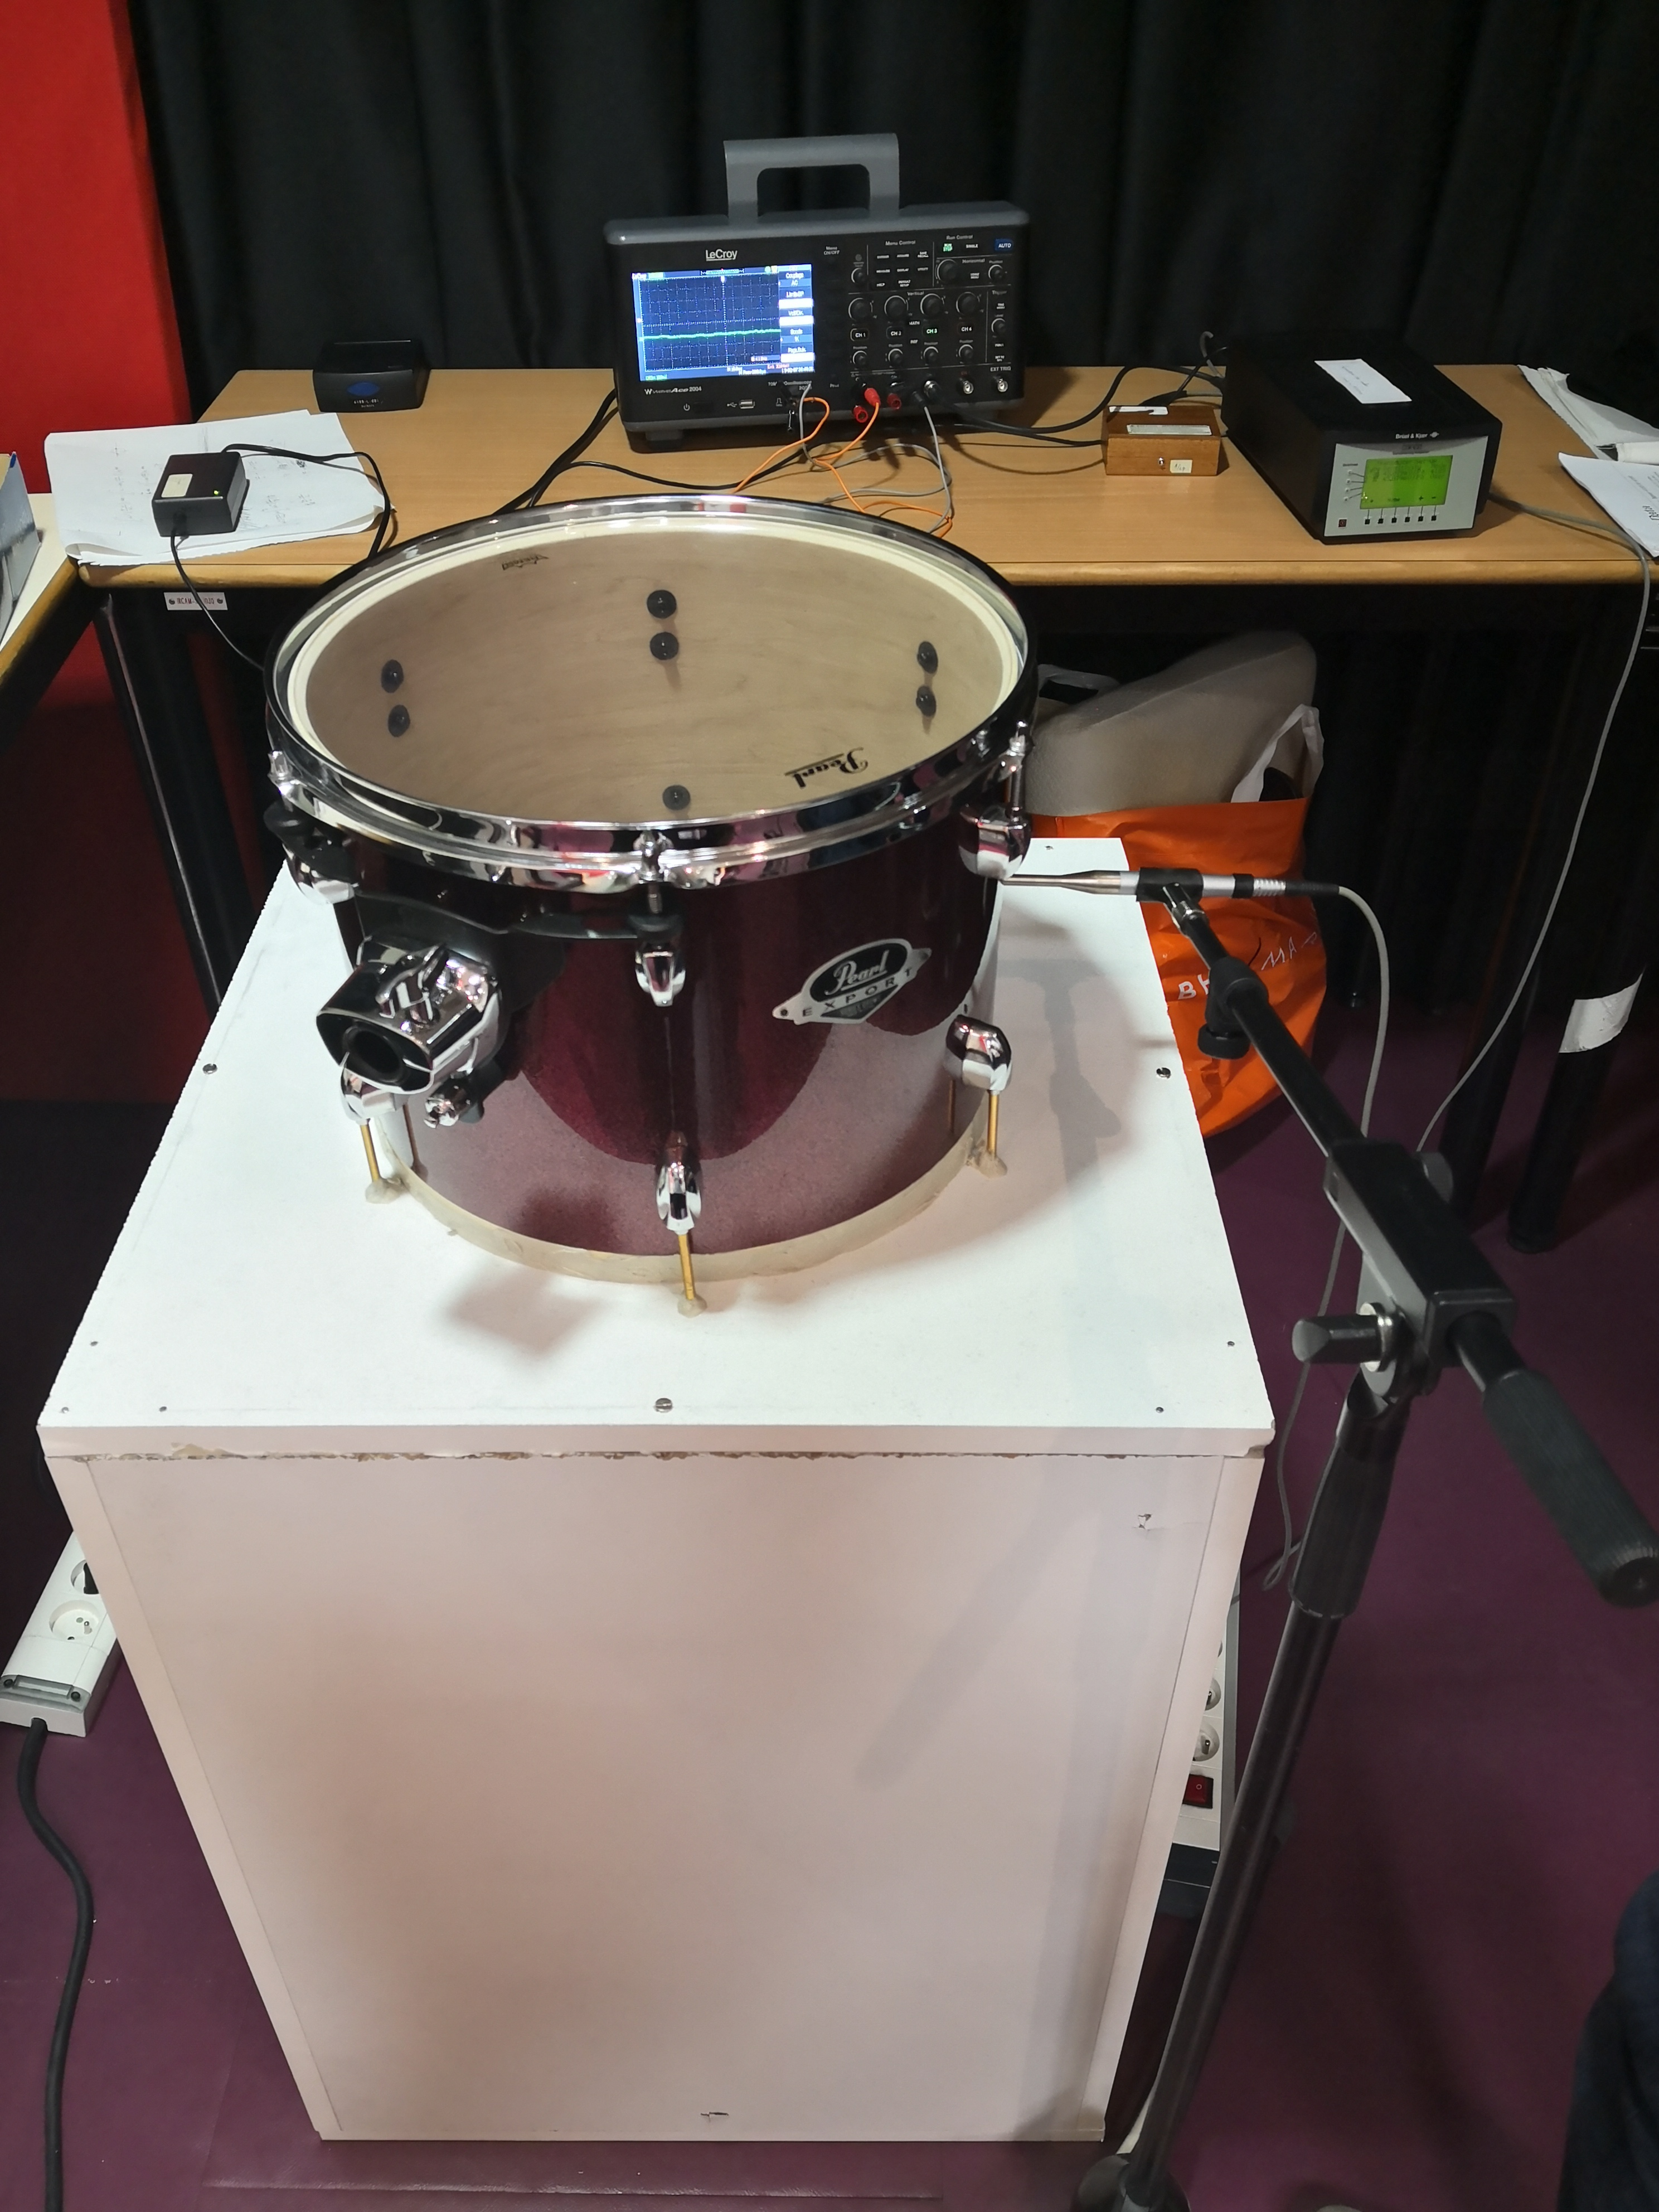
\includegraphics[width = 0.4\linewidth]{IMG_pic.jpg}
    \caption{Overall system}
\end{figure}

\begin{figure}[H]
    \centering
    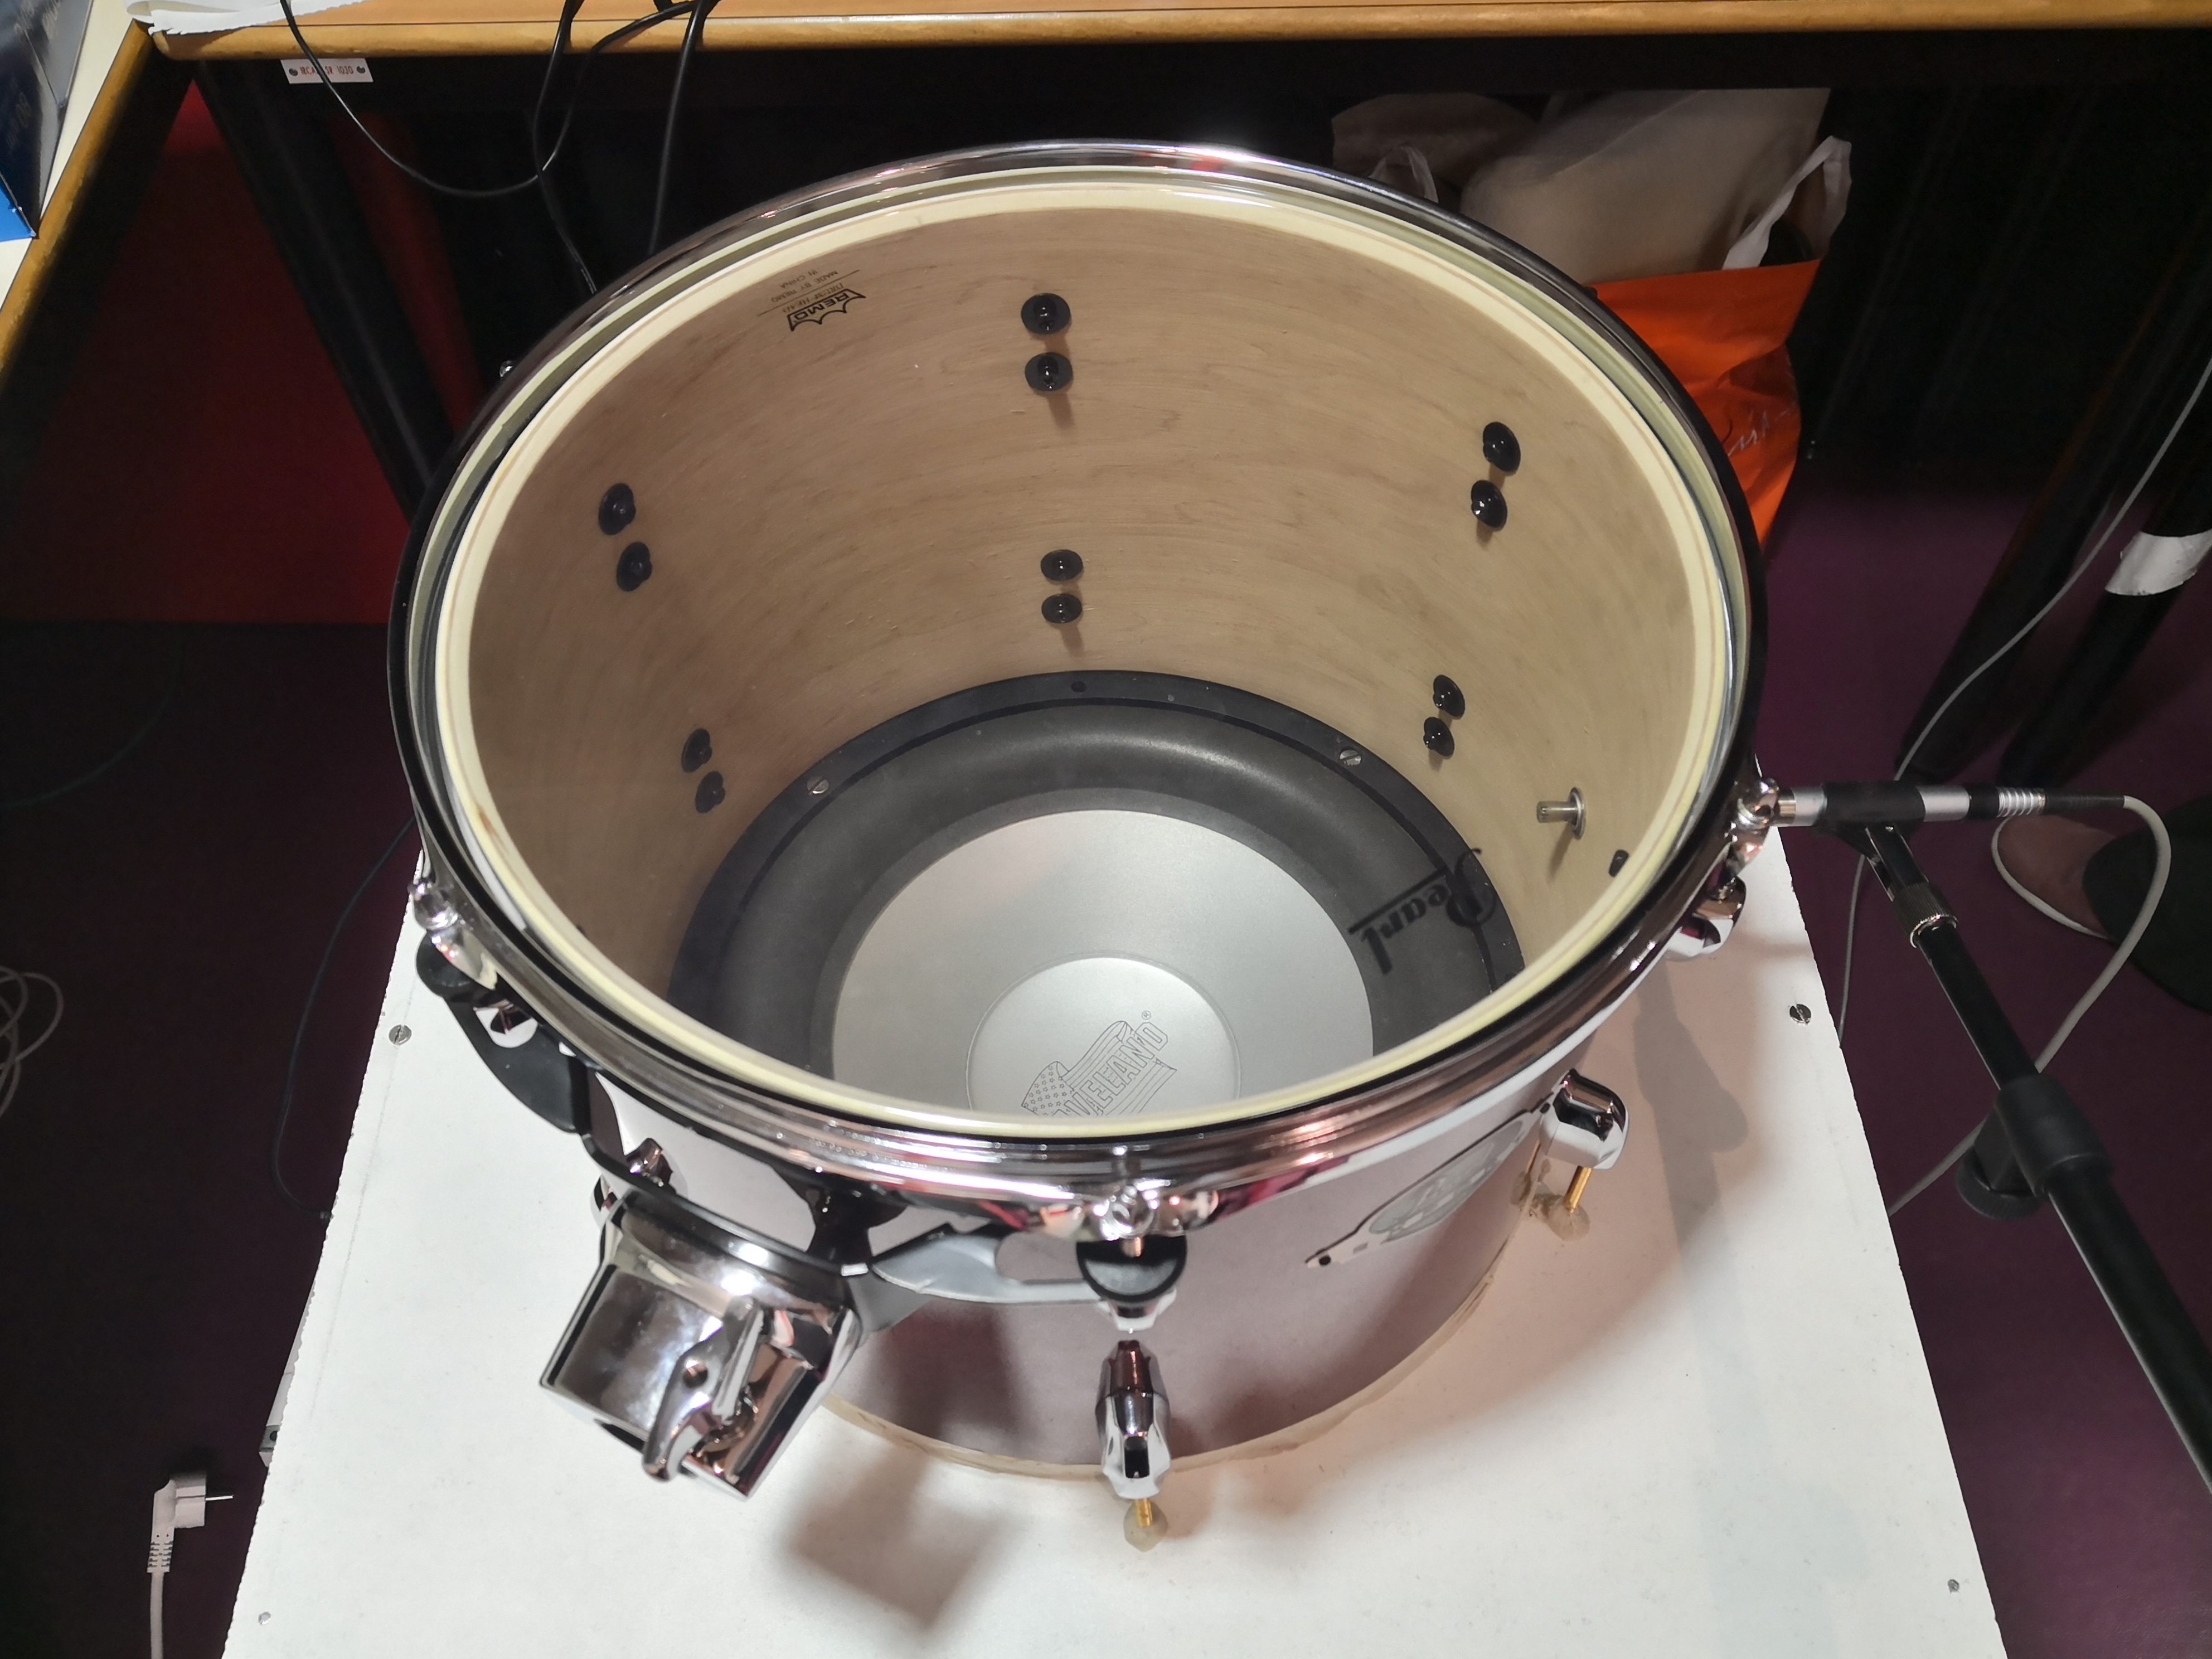
\includegraphics[width = 0.4\linewidth]{IMG_pic2.jpg}
    \caption{Zoom on the tom drum, the loudspeaker and the microphone}
\end{figure}

\end{appendix}

\end{document}
